\documentclass[20pt]{article}

%=================================================================================================
%Packages
\usepackage[spanish]{babel}
\usepackage{geometry}
\usepackage{filecontents}
\usepackage{graphicx}
\usepackage{background}
\usepackage{blindtext}
\usepackage{xcolor}
\usepackage[absolute,overlay]{textpos}
\usepackage{helvet} % PSNFSS Font, in every TeX distribution
\usepackage{parskip}
\usepackage{tcolorbox}
\renewcommand{\familydefault}{\sfdefault}
%=================================================================================================
%End of Packages


\graphicspath{{images/}}
\geometry{
	a4paper,
	total={170mm,257mm},
	left=20mm,
	top=20mm,
}

\backgroundsetup{scale = 1, angle = 0, opacity = 1,
	contents = {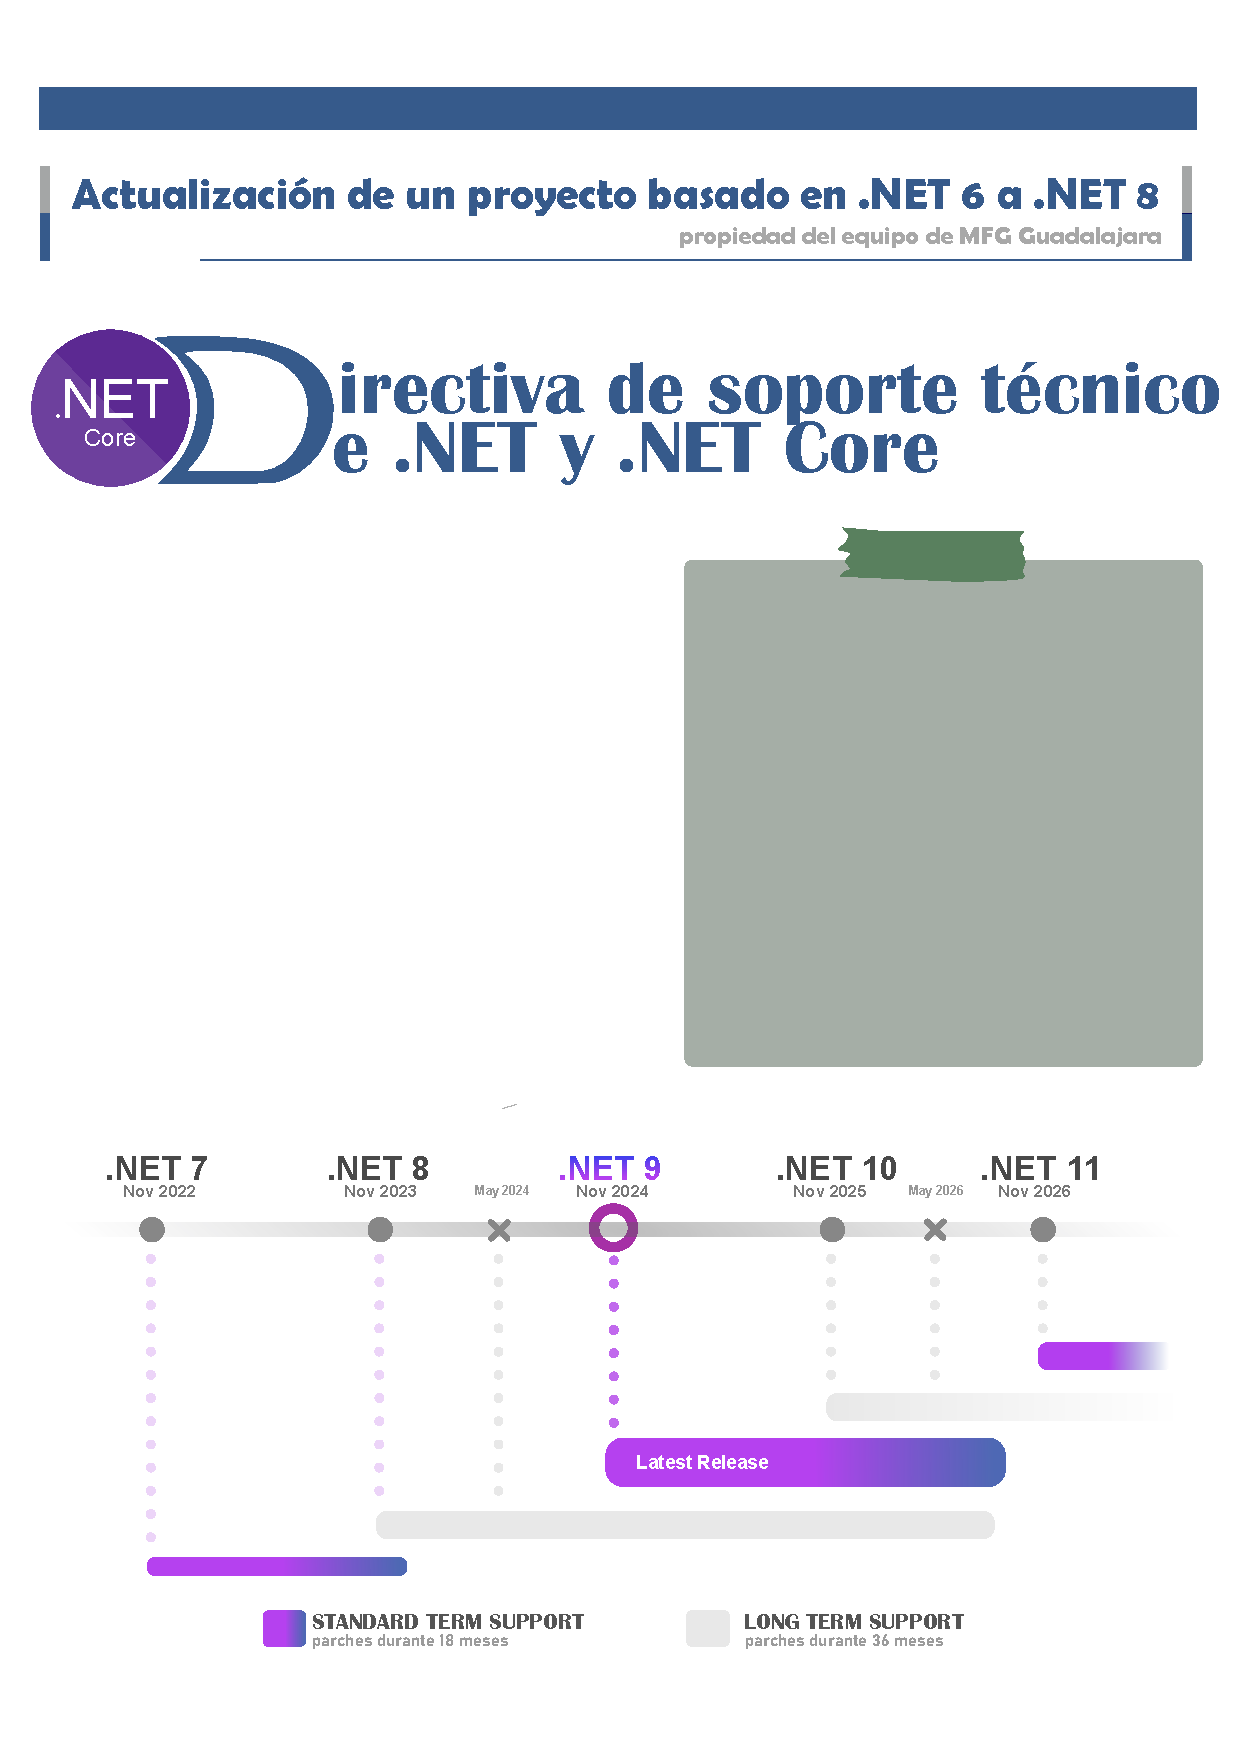
\includegraphics[width = \paperwidth,
		height = \paperheight, keepaspectratio]
		{background.pdf}}}

\begin{document}
	\fontsize{12}{13.5}\selectfont
	
	\begin{textblock*}{10cm}(1cm,10cm) % {block width} (coords) 
		Cada producto de Microsoft tiene un ciclo de vida. El ciclo de vida comienza cuando se publica un producto y finaliza cuando deja de ser compatible. Conocer las fechas clave de este ciclo de vida le ayuda a tomar decisiones informadas sobre cuándo actualizar o realizar otros cambios de software. 
		
		 \noindent El ciclo de vida de soporte técnico de .NET y .NET Core ofrece soporte para cada versión. La duración y el grado de soporte varían en función de algunas cualificaciones. 
		 
		 \noindent Los clientes pueden elegir versiones de soporte técnico de largo plazo LTS (\textbf{Long Term Support}) o versiones de soporte técnico de términos estándar STS (Standard Term Support). Las versiones LTS obtienen soporte y revisiones gratuitas durante 3 años.
	\end{textblock*}
	
		\begin{textblock*}{8cm}(12cm,10cm) % {block width} (coords) 
			\textcolor{white}{Las versiones STS obtienen soporte y revisiones gratuitas durante 18 meses.}\\
				
			\textcolor{white}{Cada año se publica una nueva versión principal de .NET en noviembre, lo que permite a los desarollaldores, la comunidad y las empresass planear sus planes de desarrollo.} \\
				
			\textcolor{white}{Las versiones con numeración impar son versiones STS que obtienen soporte técnico gratuito y revisiones durante 18 meses.}
				
			\textcolor{white}{Las versiones de LTS se admiten durante tres años después de la versión inicial.}
	\end{textblock*}
\end{document}